\documentclass[a4paper,12pt,parskip,bibtotoc,liststotoc]{article}
    %Festlegung der Dokumentenklasse, zahlreiche Vereinbarungen über Layout, Gliederungsstrukturen,
    %bsp. article -> section, subsection..., book -> chapter, section...
    %parskip = Abstand zwischen Absätzen, Veränderung durch \setlength
\usepackage[utf8]{inputenc}   %Eingabezeichencodierung, die direkte Tastatureingabe von Umlauten ist möglich
\usepackage[ngerman]{babel}     %Neu deutsche Rechtschreibung, Umlaute können geschrieben werden
\usepackage{setspace}           %für Zeilenabstand
\usepackage[notindex,nottoc]{tocbibind}   %Inhaltsverzeichnisse erstellen

%zusätzliche benötigte Pakete
\usepackage{graphicx}           %Graphik
\usepackage{amsmath,amssymb}    %Mathematik
\usepackage{natbib}             %Zitate
\usepackage{marvosym}           %enthält Symbole wie das Eurozeichen
\usepackage{eurosym}
%\setcounter{secnumdepth}{3}
%\setcounter{tocdepth}{3}
\usepackage{footmisc}
\usepackage{listings}
\usepackage{color}
\usepackage{textcomp}
\definecolor{listinggray}{gray}{0.9}
\definecolor{lbcolor}{rgb}{0.9,0.9,0.9}
\lstdefinestyle{befehl}{
	backgroundcolor=\color{lbcolor},
	tabsize=4,
	rulecolor=,
	language=ruby,
        upquote=true,
        aboveskip={1.5\baselineskip},
        columns=fixed,
        showstringspaces=false,
        extendedchars=true,
        breaklines=true,
        prebreak = \raisebox{0ex}[0ex][0ex]{\ensuremath{\hookleftarrow}},
        showtabs=false,
        showspaces=false,
        showstringspaces=false,
        identifierstyle=\ttfamily,
        keywordstyle=\color[rgb]{0,0,1},
        commentstyle=\color[rgb]{0.133,0.545,0.133},
        stringstyle=\color[rgb]{0.627,0.126,0.941}
}

\lstdefinestyle{Listing}{
	frame=single,
	tabsize=4,
	rulecolor=,
	language=ruby,
        upquote=true,
        aboveskip={1.5\baselineskip},
        columns=fixed,
        showstringspaces=false,
        extendedchars=true,
        breaklines=true,
        prebreak = \raisebox{0ex}[0ex][0ex]{\ensuremath{\hookleftarrow}},
        showtabs=false,
        showspaces=false,
        showstringspaces=false,
        identifierstyle=\ttfamily,
        keywordstyle=\color[rgb]{0,0,1},
        commentstyle=\color[rgb]{0.133,0.545,0.133},
        stringstyle=\color[rgb]{0.627,0.126,0.941}
}


\usepackage{amsmath}
%\usepackage{mathtools} % lädt auch amsmath
\usepackage{moreverb}

\usepackage{amsthm}
\newtheorem{mydef}{Definition}

\usepackage[table]{xcolor}
\usepackage{colortbl}
\usepackage{multirow}
\usepackage{mdwlist}   %Verringerung Abstand zwischen items -> \begin{itemize*} \end{itemize*}
\usepackage[labelsep=space,justification=centering]{caption}

%\usepackage{hyperref}  %erlaubt Links innerhalb des pdf-Dokuments zu erzeugen

\setlength{\parindent}{0pt}     %Verhinderung des horizontalen Einrückens zu Beginn eines Absatzes

%Seitenlayout
\topmargin -0.9cm       %Vertikaler Abstand der Kopfzeile von der Bezugslinie
\textheight 25cm        %Abstand der Grundlinie der Kopfzeile zum Haupttext
\textwidth 16.5cm       %Breite des Haupttexts
\footskip 1cm           %Abstand der Grundlinien der letzten Textzeile und der Fußzeile
\voffset -0.5cm         %Vertikale Bezugspunktposition
\hoffset -1.2cm         %Horizontale Bezugspunktposition

\onehalfspacing         %anderthalbzeiliger Abstand

\newcommand{\url}{\;}   %URL im Literaturverzeichnis

%eigene Befehlsdefinitionen
\newcommand{\be}{\begin{equation}}     %Mathematische Umgebung
\newcommand{\ee}{\end{equation}}
\newcommand{\bea}{\begin{eqnarray}}
\newcommand{\eea}{\end{eqnarray}}
\newcommand{\bean}{\begin{eqnarray*}}  %ohne Nummerierung
\newcommand{\eean}{\end{eqnarray*}}    %ohne Nummerierung
%%%%%%%%%%%%%%%%%%%%%%%%%%%%%%%%%%%%%%%%%%%%%%%%%%


%%%%%%%%%%%%%%%%%%%%%%%%%%%%%%%%%%%%%%%%%%%%%%%%%%%%%%
%
%    Anfang des Textes
%
%%%%%%%%%%%%%%%%%%%%%%%%%%%%%%%%%%%%%%%%%%%%%%%%%%%%%%
\begin{document}

\pagenumbering{roman}  %römische Seitennummerierung
%%%%%%%%%%%%%%%%%%%%%%%%%%%%%%%%%%%%%%%%%%%%%%%%%%%%%%
%
%    Titelseite
%
%%%%%%%%%%%%%%%%%%%%%%%%%%%%%%%%%%%%%%%%%%%%%%%%%%%%%%
\thispagestyle{empty}  %keine Seitenzahl auf Titelseite
Leibniz Universität Hannover\\
Wirtschaftswissenschaftliche Fakultät\\
Institut für Produktionswirtschaft\\
Prof.\ Dr.\ Stefan Helber

\vspace{5cm}

\begin{center}
Hausarbeit im Rahmen der Veranstaltung \\
Entwicklung von Anwendungssystemen  im WiSe 2014/2015 \\
(Veranstaltungs-Nr. 173610)

\vspace{2.5cm}

%Thema Nr. 5\\[1mm]    %hier Themennummer eintragen
{\Large RCPSP \\
RCPSP}
\end{center}

\vspace{5.5cm}


\begin{table}[h!]
    \vspace*{-3mm}
    \hspace*{2mm}
  \renewcommand{\arraystretch}{1,5}
    \begin{tabular}{ll}
Andreas Hipp &Robert Matern \\
Ungerstr. 24&Plathnerstr. 49 \\
30451 Hannover&30175 Hannover \\
Matr.-Nr. 3027520 ???&Matr.-Nr. 2798160 \\[3mm]
Abgabedatum: 24.03.2015
	\end{tabular}
\end{table}

\newpage

%Inhaltsverzeichnis erstellen
\tableofcontents

\newpage  %neue Seite

%Abbildungsverzeichnis erstellen
\listoffigures

%Tabellenverzeichnis erstellen
\listoftables

%Codeverzeichnis
\renewcommand\lstlistlistingname{Quellcodeverzeichnis} 
\lstlistoflistings 
\renewcommand*\lstlistingname{Quellcode} 

\newpage
%Abkürzungsverzeichnis
\section*{Abkürzungsverzeichnis}
\addcontentsline{toc}{section}{Abkürzungsverzeichnis}
\begin{table}[h!]
    \vspace*{-3mm}
    \hspace*{2mm}
  \renewcommand{\arraystretch}{1,5}
    \begin{tabular}{ll}  %hier die Spaltenausrichtung und Anzahl eintragen
           RCPSP      & Resource-Constrained Project Scheduling \\
           RoR & Ruby on Rails \\
SGS & Schedule Generation Scheme\\
	\end{tabular}
\end{table}
\newpage
%Symbolverzeichnis
\section*{Symbolverzeichnis}
\addcontentsline{toc}{section}{Symbolverzeichnis}
\begin{table}[h!]
    \vspace*{-3mm}
        \hspace*{2mm}
      \renewcommand{\arraystretch}{1,5}
    \begin{tabular}{ll} 
$d_i$ & Dauer von Vorgang $i$ \\
$FE_i$& frühestes Ende von Vorgang $i$\\
$i,h=1,...,I$ & Vorgänge \\
$k_{ir}$& Kapazitätsbedarf von Vorgang $i$ auf Ressource $r$\\
$kp_r$ & verfügbare Kapazität von Ressource $r$ je Periode\\
$\mathcal{N}_i$ & Menge der direkten Nachfolger von Vorgang $i$ \\
$oc_r$ & Kosten einer Einheit Zusatzkapazität von Ressource $r$ \\
$O_{rt}$ & Zusatzkapazität von Ressource $r$ in Periode $t$ \\
$r=1,...,R$ & Ressourcen \\
$SE_i$& spätestes Ende von Vorgang $i$\\
$t,\tau=1,..., T$ & Perioden\\
$\mathcal{V}_i$ & Menge der direkten Vorgänger von Vorgang $i$ \\
$X_{jt}\in\{0,1\}$ & gleich $1$, falls Vorgang $j$ in Periode $t$ endet, sonst $0$
  	\end{tabular}
\end{table}
\newpage
\pagenumbering{arabic}   %ab hier arabische Seitenzahlen beginnend mit 1

%%%%%%%%%%%%%%%%%%%%%%Textteil%%%%%%%%%%%%%%%%%%%%%%%%%%

\section{Einleitung} \label{start}
%Bereits seit mehreren Dekaden spielt Projektarbeit eine wichtige Rolle bei der Aufgabenabwicklung in Wirtschaft und Verwaltung.\footnote{Vgl. \cite{zimmermann2006projektplanung}, S. VI}
Bei einem Projekt handelt es sich um eine zeitlich befristete, relativ innovative und risikobehaftete Aufgabe von erheblicher Komplexität, die meist einer gesonderten Planung bedarf.\footnote{Vgl. \cite{projektdef}} Dementsprechend von großer Bedeutung ist die vorhergehende und genaue Planung von Projekten.\footnote{Vgl. \cite{zimmermann2006projektplanung}, S. VI\label{zum}} Projektplanung ist die Planung aller Arbeitsgänge eines Projekts durch Zuweisung eines Startzeitpunktes, so dass die Zeitbeziehung zwischen den Vorgängen eingehalten und knappe Ressourcenkapazitäten nicht überschritten werden.\footref{zum} Durch das Zerlegen des Projekts in einzelne Arbeitsgänge wird versucht die Komplexität zu reduzieren und eine geordnete Abfolge der Arbeitsgänge zu erstellen, um das Projektziel zu erreichen.\footnote{Vgl. \cite{zimmermann2006projektplanung}, S. 4} Projektziele können dabei unterschiedlich kategorisiert werden, z. B. in Sach-, Termin- oder Kostenziele.\footnote{Vgl. \cite{felkai2011analysieren}, S. 52}\\

Nach DIN 69900 hat ein Arbeitsgang oder ein einzelner Vorgang eines Projekts einen definierten Anfang sowie ein definiertes Ende und dient für das Projekt als Ablaufelement zur Beschreibung eines bestimmten Geschehens.\footnote{Vgl. \cite{69900D}, S. 15} Trotz der Zerlegung besitzen die einzelnen Arbeitsgänge des Projekts eine Beziehung, mit der die Reihenfolge der Ablauffolge bestimmbar ist.\footnote{Vgl. \cite{kellenbrink2014einfuhrung}, S. 6-7} Oft wird zur Darstellung der Vorgangsbeziehung ein Vorgangsknoten-Netzplan verwendet.\footnote{?????} %D. h. es können nur Arbeitsgänge abgeschlossen werden, wenn deren notwendigen Vorgänge bereits abgeschlossen wurden. Ein einfaches Beispiel wäre die sogenannte Hochzeit in der Automobilherstellung. Sobald Karosserie und Motor eines Fahrzeugs hergestellt wurden, können diese zwei Elemente in einem nachfolgenden Prozess verbunden werden.
Ein Arbeitsgang ist i. d. R. verbunden mit dem Einsatz von Ressourcen, welche wiederum mit Kosten verbunden sind. Eine Möglichkeit, das Projektziel unter minimaler Ressourcenverwendung zu erreichen, ist die effiziente Planung der Ablauffolge der Arbeitsgänge eines Projekts.\footnote{Vgl. \cite{bartels2009projektplanung}, S. 11-12} Damit ist es möglich, mehrere Projekte bei einer gegebenen Zeitvorgabe unter Einhaltung von Ressourcenrestriktionen fertigzustellen bzw. bei konstanter Ressourcenkapazität ein Projekt in kürzerer Zeit abzuschließen. \\

%Dementsprechend versucht eine effiziente Projektplanung, neben der Einhaltung des Projektziels, auch den Einsatz der Ressourcen zu minimieren.\footnote{Vgl. \cite{bartels2009projektplanung}, S. 11-12}  %Projektmanagement, neben der Einhaltung des Projektziels, auch den Einsatz der Ressourcen zu minimieren.\footnote{Vgl. \cite{bartels2009projektplanung}, S. 11-12}


%\begin{mydef}
%\glqq Allgemein bezeichnet der Begriff Projektmanagement alle leitenden und administrativen Aktivitäten, die zur Durchführung eines Projektes notwendig sind. Es beschreibt die Gesamtheit von Führungsaufgaben, -organi\-sation, -techniken und -mitteln zur zielorientierten Durchführung großer Vorhaben.\grqq\footnote{Vgl. \cite{hering2014projektmanagement}, S. 1-3; in Anlehnung an DIN 69901 und ISO 21500:2012-09}
%\end{mydef}

%Beispielweise kann ein Automobilhersteller durch Optimierung des Produktentstehungsprozess durch effizientes planen seiner vorhandenen Ressourcen in einer vordefinierten Zeit eine größere Anzahl an Fahrzeugen entwickeln, als wenn das Unternehmen keine effiziente Projektplanung verfolgt. 

%Eine effiziente Projektplanung reduziert die gesamte Fertigstellungsdauer eines Projekts. Es wird eine wirkungsvolle Gestaltung des Verbrauchs der zur Verfügung stehenden Ressourcen über die Laufzeit des Projekts ermöglicht. Somit handelt es sich um ein mathematisches Optimierungsproblem, bei dem für ein Projekt die Ressourcenbeschränkung über die Laufzeit einzuhalten ist und die Fertigstellungszeit minimiert werden soll.
%Für das ressourcenbeschränkte Projektplanungsproblem gibt es Verfahren der exakten und heuristischen Lösung. In der Praxis, wie auch in dieser Arbeit \footnote{Vgl. Kapitel \ref{notwendig}}, wird i. d. R. auf Heuristiken zurückgegriffen.\footnote{Vgl. \cite{herroelen2005project}, S. 420}
%Eine typische Ressource in der Projektplanung ist der Faktor Zeit, da lt. Definition ein Projekt zeitlich befristet ist. % Andere Arten von Ressourcen sind dürfen bei der Planung von Projekten jedoch nicht vernachlässigt werden.
Zur Bestimmung der optimalen Ablauffolge der einzelnen Arbeitsgänge eines Projekts kann ein Optimierungsmodell verwendet werden, bei der für eine festgelegten Ablauffolge eines Projekts und unter Berücksichtigung der Ressourcenbeschränkung die Fertigstellungszeit minimiert wird. Im Kapitel \ref{Grund} wird eine solche Modellformulierung für das ressourcenbeschränkte Projektplanungsproblem als sogenannte Kapazitätsplanung vorgestellt.\footnote{????} Alternativ wird in dem Kapitel das Optimierungsmodell um die Bedienung erweitert, dass  Zusatzkapazitätseinheiten gebucht werden können. Mit dieser Modellerweiterung wird von der Kostenplanung in Projekten gesprochen. Bezeichnet wird im Allgemeinen das ressourcen-beschränkte Projektplanungsproblem  mit der englischen Bezeichnung des \textit{Resource-Constrained Project Scheduling Problem (RCPSP)}. Bei dem RCPSP handelt es sich um eine abstrakte mathematische Modellformulierung. Ziel der vorliegenden Arbeit ist es das RCPSP in Ruby on Rails (RoR) zu implementieren. Bei RoR handelt es sich um ein Framework zur Entwicklung von Webdokumenten bzw. Internetseiten.\footnote{???} Es baut auf der Programmiersprache Ruby auf und ist ursprünglich von David Heinemeier Hansson entwickelt.\footnote{???} Die Implementierung bedarf einer Verknüpfung von RoR und GAMS\footnote{General Algebraic Modeling System}. Unter GAMS wird eine algebraische Modellierungssprache für mathematische Optimierungsprobleme verstanden, mit der das RCPSP gelöst wird.\footnote{???} Im Kapitel \ref{Haupt} wird die Entwicklung des Anwendungssystems zum Lösen des RCPSP ausführlich beschrieben. Ergänzt wird diese Arbeit durch eine kritische Würdigung des Anwendungssystems in Kapitel \ref{krit} sowie einem Fazit in Kapitel \ref{Fazit}.

\section{Grundlagen zur ressourcen-beschränkten Projektplanung und zu dem Framework Ruby on Rails} \label{Grund}
\subsection{Kapazitätsplanung}
Ein Großteill an Projekten besitzt die Eigenschaft eines beschränkten Ressourcenkontingents.\footnote{Vgl. \cite{kellenbrink2014einfuhrung}, S. 11} Soll demgemäß die vorgegebene Terminierung des Projektes als zuvor festgesetztes Ziel erreicht werden, muss neben der Reihenfolgerestriktion auch der Ressourcenbedarf der unterschiedlichen Arbeitsgänge sichergestellt werden. Mit der Einhaltung des Ressourcenbedarfs ist es möglich, alle zur Erfüllung des Projektes notwendigen Arbeitsgänge auszuführen und somit letztendlich das Projekt abzuschließen. Neben limitierten Ressourcen, die während des gesamten Projekts nur ein Mal zur Verfügung stehen, wie bspw. das Projektbudget, gibt es Ressourcen, die nach einer bestimmten Anzahl von Perioden erneuert werden können.\footnote{Vgl. \cite{neumann2003project}, S. 21-22} Erneuerbare Ressourcen sind bspw. die Produktionskapazität einer Maschine oder der Personaleinsatz für ein Projekt. In dieser Arbeit wird der Fokus auf diese erneuerbaren Ressourcen gelegt.\\

Zur Lösung des ressourcenbeschränkten Projektplanungsproblems kann das Modell RCPSP genutzt werden. Das RCPSP legt durch Fixierung der Aktivitätsstartzeitpunkte den Projektgrundablauf zur Zielerreichung der Minimierung der Projektdauer fest. Dies geschieht unter Einhaltung der Startzeitpunkt- bzw. der Vorrangsbedingung der einzelnen Arbeitsgänge sowie der Kapazitätsbeschränkung der erneuerbaren Ressourcen.\footnote{Vgl. \cite{demeulemeester2011robust}, S. 23} Die im folgenden aufgestellte Zielfunktion des RCPSP zur Minimierung der Projektdauer ist die gängige Version der Kapazitätsplanung,\footnote{Vgl. \cite{drexl1997neuere}, S. 98} andere Variationen sind aber ebenfalls möglich.\footnote{Vgl. \cite{talbot1982resource}, S. 1200}\\

Nachfolgend wird das deterministische RCPSP in diskreter Zeit formuliert.\footnote{????} Charakteristisch für eine mathematische Modellformulierung in diskreter Zeit sind die Zeiteinheiten, die den Perioden $t, \tau$ entsprechen.\\

\textbf{Modell RCPSP}
\begin{eqnarray} \label{Ziel}
\min Z = \sum_{t=FE_{I}}^{SE_{I}}t \cdot X_{I,t}\hfill  
\end{eqnarray}

unter Beachtung der Restriktionen
\begin{multline} \label{N1}
\sum_{t=FE_{i}}^{SE_{i}} X_{it} = 1
\hfill   i = 1,...,I
\end{multline}\vspace{-3.0ex}

\begin{multline} \label{N2}
\sum_{t=FE_{h}}^{SE_{h}}t \cdot X_{ht} \leq \sum_{t=FE_{i}}^{SE_{i}}(t - d_{i}) \cdot X_{it}
\hfill   i =1,...,I;\; h \in \mathcal{V}_{i}
\end{multline}\vspace{-3.0ex}

\begin{multline} \label{N3}
\sum_{i=1}^{I}\sum_{\tau=\max(t,FE_{i})}^{\tau=\min(t+d_i-1,SE_i)}k_ {ir} \cdot X_{i\tau} \leq kp_{r}
\hfill   r =1,...,R;\; t=1,...,T
\end{multline}\vspace{-3.0ex}
\begin{multline} \label{N4}
X_{it} \in \{0,1\}
\hfill   i \in \mathcal{I};\; t \in \{FE_{i},...,SE_{i}\}\end{multline}\vspace{-6.0ex}\\

Es wird ein Projekt betrachtet, dass aus $I$ unterschiedlichen Arbeitsgängen besteht. Jeder Arbeitsgang $i$ hat eine definierte Menge von zu erledigenden Vorgängerarbeitsgängen $h \in \mathcal{V}_{i}$. Des Weiteren ist für die Fertigstellung des Projekts die Abarbeitung der Arbeitsgänge in topologischer Reihenfolge notwendig. D. h. der Vorgänger $h$ hat stets eine kleinere Ordnungszahl als sein Nachfolger $i\;(h<i)$ und muss zur Fortsetzung des Projektverlaufs beendet sein. Die Bearbeitungsdauer eines Arbeitsgangs $i$ wird mit dem Parameter $d_{i}$ festgelegt.  Bei dem RCPSP in diskreter Zeit wird die Annahme getroffen, dass die Dauer durch einen ganzzahligen Parameter abgebildet wird. Der Startzeitpunkt des Projekts ist $t = 0$ und erstreckt sich über einen Gesamtzeitraum von $T$ Perioden. Um die Reihenfolgebedingungen einzuhalten, werden einem Projekt zwei Dummy-Arbeitsgänge \glqq Beginn\grqq\;($i=1$) und \glqq Ende\grqq\;($i=I$) hinzugefügt, welche mit einer Dauer von $0$ Zeiteinheiten bewertet werden.\footnote{Vgl. \cite{zimmermann2006projektplanung}, S. 66} Dadurch wird der Projektbeginn und das Projektende exakt terminiert. Der Parameter $k_{ir}$ stellt die benötigten Kapazitäten der erneuerbaren Ressource $r$ bei der Durchführung von Arbeitsgang $i$ dar. Die Ressourcen $r \in R$ sind in einer Periode innerhalb des Umfangs ihrer Kapazität $kp_{r}$ nutzbar. Da es sich um erneuerbare Ressourcen handelt, stehen diese zu jeder neuen Periode in vollem Umfang erneut zur Verfügung. Ungenutzte Ressourcen sind jedoch nicht auf nachfolgende Arbeitsgänge und Perioden übertragbar.\footnote{Vgl. \cite{kellenbrink2014einfuhrung}, S. 12} Um den Fertigstellungszeitpunkt der einzelnen Arbeitsgänge $i$ festlegen zu können, wird der Modellformulierung in diskreter Zeit die binäre Entscheidungsvariable $X_{it}$ hinzugefügt.\footnote{Vgl. \cite{pritsker1969multiproject}, S. 94} Diese Binärvariable nimmt den Wert $1$ an, falls der Arbeitsgang $i$ zum Zeitpunkt $t$ beendet wird.\\

Mittels der Zielfunktion \eqref{Ziel} wird der Fertigstellungszeitpunkt des Projekts minimiert. Dafür wird der Zeitraum zwischen dem frühesten und spätesten Fertigstellungszeitpunkt $FE_{I}$ und $SE_{I}$ aller durchzuführenden Arbeitsgänge $I$ betrachtet. Nebenbedingung \eqref{N1} stellt sicher, dass ein Arbeitsgang $i$ zwischen dem jeweiligen für diesen Arbeitsgang geltenden frühesten und spätesten Fertigstellungszeitpunkt nur exakt ein Mal durchgeführt wird. Die Reihenfolgerestriktion wird mit der Nebenbedingung \eqref{N2} eingehalten. Sie stellt sicher, dass jeder Vorgänger $h \in \mathcal{V}_{i}$ beendet ist, bevor der Arbeitsgang $i$ startet. Der Term $(t - d_{i})$ garantiert für den Arbeitsgang $i$, dass dieser erst beginnt, sobald der Vorgänger $h$ mit der Dauer $d_{i}$ abgeschlossen ist.
Der Parameter $kp_{r}$ spiegelt die Kapazitätsgrenze für eine erneuerbare Ressource $r$ je Periode $t$ wieder. In Nebenbedingung \eqref{N3} findet zum einen eine formale Darstellung dieser Kapaiztätsbegrenzung statt. Zum anderen wird der Ressourcenverzehr während der gesamten Bearbeitungsdauer der Fertigstellung beachtet, in dem der Kapazitätsbedarf $k_{ir}$ aller Arbeitsgänge $I$ summiert wird. Eben diese Summe wird schließlich durch $kp_{r}$ beschränkt. %????Da ist irgendwas falsch...
Mit der Nebenbedingung \eqref{N4} wird die Binärvariable $X_{it}$ für den Zeitraum $t = \{FE_{i},...,SE_{i}\}$ formal definiert. Aufgrund der Reihenfolgebeziehung \eqref{N2} darf der jeweils betrachtete Arbeitsgang nur in diesem Zeitraum fertiggestellt werden.
Die gemischt-ganzzahlige Modellformulierung lässt sich durch Standard-Lösungsverfahren exakt lösen.\footnote{z. B. mittels eines Branch-and-Bound-Verfahrens, Vgl. \cite{kellenbrink2014einfuhrung}, S. 14}

\subsection{Kostenplanung}
Aufbauen auf der Kapazitätsplanung kann das RCPSP um die Nutzung von Zusatzkapazitäten der Ressourcen erweitert werden, damit dem Projektplanungsmodell gestattet ist den Vorgänge zusätzliche Kapazitätseinheiten der notwendigen Ressourcen bereitzustellen. Die Kapazitätsrestriktion wird dementsprechend um die Entscheidungsvariable $O_{rt} \geq 0$ erweitert. Die Variable $O_{rt}$ beschreibt die Einheiten an Zusatzkapazitäten einer Ressource $r$ in der Periode $t$. Damit steht nicht die Einhaltung der verfügbaren Kapazitäten im Vordergrund, sonder unter Beachtung der Projektstruktur die aufgewendeten Zusatzkosten des Projekts. Dem Optimierungsmodell ist es damit gestattet durch Erhöhung der Kapazitäten der Ressourcen die anfängliche Ressourcenbeschränkung zu umgehen. Bei der Modellerweiterung der Kostenplanung wird der Parameter $oc_r$ eingeführt, der für eine betrachtete Ressource $r$ die Kosten einer Einheit der Zusatzkapazitäten beschreibt. Ziel des Optimierungsmodells ist es damit die Kosten des Projekts zu minimieren. Das Modell hilft damit der Entscheidung, ob durch Einführen der Möglichkeit von Zusatzkapazitäten das Projektziel verbessert erreicht wird. Es handelt sich um den Trade-off des frühzeitigen Erreichens des Projektziels durch Nutzung von Zusatzkapazitäten und der gesamten Projektkosten die für das Projekt aufgewendet werden sollen.\\

Nachfolgend wird das deterministische RCPSP+ in diskreter Zeit formuliert.

\textbf{Modell RCPSP+}
\begin{eqnarray} \label{Ziel2}
\min Z = \sum_{t=1}^{T}\sum_{t=1}^{R} oc_{r} \cdot O_{r,t}\hfill  
\end{eqnarray}

unter Beachtung der Restriktionen \eqref{N1}, \eqref{N2}, \eqref{N4} sowie
\begin{multline} \label{N5}
\sum_{i=1}^{I}\sum_{\tau=\max(t,FE_{i})}^{\tau=\min(t+d_i-1,SE_i)}k_ {ir} \cdot X_{i\tau} \leq kp_{r} + O_{rt}
\hfill   r =1,...,R;\; t=1,...,T
\end{multline}\vspace{-3.0ex}
\begin{multline} \label{N6}
O_{rt} \geq 0
\hfill   r =1,...,R;\; t=1,...,T \end{multline}\vspace{-6.0ex}\\

Bei dem RCPSP+ wird die Zielfunktion insoweit formuliert, dass über alle Perioden $t\in T$ und über alle Ressourcen $r\in R$ die Summe der Kosten $oc_r$ für die Anzahl an notwendige Einheiten an Zusatzkapazität $O_{rt}$ minimiert wird. Weiterhin bleibt die Nebenbedienung \eqref{N1} und \eqref{N2} bestehen, dass jeder Vorgang exakt einmal zwischen dem frühesten Ende ($FE_i$) und dem spätesten ($SE_i$) fertiggestellt und die Topologie der Vorgänge eingehalten wird. Weiterhin gilt die Nebenbedingung \eqref{N4}, dass es sich bei der Entscheidungsvariable $X_{jt}$ um eine binäre Variable handelt. Erweitert wird das RCPSP aus der Kapazitätsplanung mit einer modifizierten Nebenbedingung zur Einhaltung Kapazitätsbeschränkung. Mit der Nebenbedingung \eqref{N5} wird die Kapazitätsrestriktion für eine Ressource $r\in R$ in einer Periode $t\in T$ eingehalten, jedoch ist es dem Modell gestattet die vorhandene Ressourcenkapazität $kp_r$ um die Ausprägung der Entscheidungsvariable $O_{rt}$ zu erweitern. Durch Lösen des Optimierungsmodells wird der Ablaufplan des Projekts unter Beachtung der unterschiedlich zulässigen Gesamtdauern $SE_I$ generiert. Weiter wird für jede Ressource $r\in R$ zur jeweiligen Periode $t\in T$ die notwendige Anzahl an benötigter Zusatzkapazität $O_{rt}$ ermittelt. Die Nebenbedingung \eqref{N6} beschreibt die Eigenschaft der Entscheidungsvariable $O_{rt}$, dass es sich um eine positive Variable bzw. einen Nullwert handelt.

\subsection{Ruby on Rails}

Das Frameworks Ruby on Rails (RoR) zur Entwicklung von Web-Applikationen mit Datenbankbezug wurde von David Heinemeier Hansson im Jahre 2004 erstmals vorgestellt.\footnote{Vgl. \cite{ruby2004}} Mit dem Name von RoR wird klar, das das Framework die Programmiersprache Ruby nutzt. Ruby wird von den den meisten gängigen Betriebssystem unterstützt (Microsoft Windows, Apple Mac OS X, Linux, etc.) und ist bspw. dem Betriebssystem Apple Mac OS X in der Version 1.8.7 standardmäßig integriert.\footnote{Vgl. \cite{ruby-schienen}} Bei Ruby handelt es sich um eine objekt-orientierte Programmiersprache mit dem Grundsatz \textit{principle of least surprise} und folgt einigen Besonderheiten, wie z. B. einer einfachen Sprachsyntax, keiner typisierten Variablen und einer reinen Objektorientierung.\footnote{Vgl. \cite{Walter:2008aa}, S. 297-298} Abbildung \ref{Terminal} zeigt das Terminal von Apple Mac OS X mit typischen Ruby Kommandobefehlen. RoR nutzt diesen einfachen Syntax zur Entwicklung von Web-Applikationen, wobei aufgrund einfacherer Bedienung auf integrierte Entwicklungsumgebung zurückgegriffen wird, wie z. B. RadRails oder RubyMine.\footnote{Vgl. \cite{hartl2012ruby}, S. 10} \\

\begin{figure}[h!]
  \begin{center}
    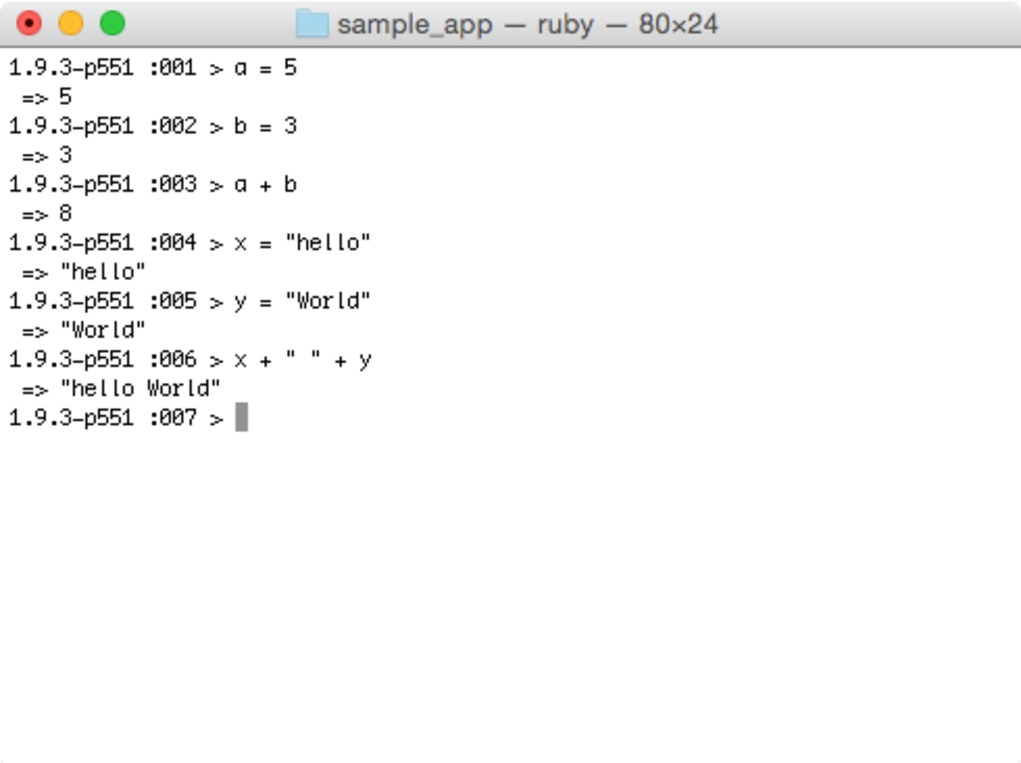
\includegraphics[width=120mm]{Bilder/Terminal.pdf}
    \caption{Terminalfenster unter Apple Mac OS X}  \label{Terminal}
  \end{center}
\end{figure}

Mit Hilfe des RoR Frameworks lassen sich dadurch schnell Web-Applikationen mit Datenbankbezug entwicklen, wobei der wesentlichen Vorteile in der Softwarearchitektur des Model-View-Controller-Paradigmas liegt.\footnote{Vgl. \cite{walter2008ruby}, S. 463} Das Paradigma besagt, dass eine durch einen Browser angestoßene Anfrage an den Server durch den Rails \texttt{controller} verarbeitet wird. Der \texttt{controller} verarbeitet die Anfrage und leitet die nachfolgenden Schritte ein. Bei Web-Applikationen erfolgt eine solche Verarbeitung durch anzeigen bzw. dem sogenannten \textit{rendern} von HTLM-Dokumenten der Rails \texttt{views} , die von Browsern angezeigt werden können. Der \texttt{controller} rendert die \texttt{views} und ermöglicht weitere RoR-Befehle im HTML-Dokument. Bei komplexen und dynamischen Seiten übernimmt der \texttt{controller} geforderte Daten aus den Rails \texttt{models}, die wiederum mit einer Datenbank verbunden sind. Durch diese Architektur lassen sind umfangreiche und an spezifische Anfrage angepasste Web-Applikationen entwickeln. Ein weiterer Vorteil von RoR ist die einfache Implementierung von Unterprogrammen. Ein Unterprogramme ist in Ruby/RoR ein \texttt{Gemfile}, das durch den Bundler zur bestehenden Web-Applikation hinzugefügt wird.\footnote{Vgl. \cite{hartl2012ruby}, S. 9-17} Im nachfolgenden Kapitel wird die Entwicklung einer Web-Applikation mittels RoR beschrieben. Dabei liegt die Besonderheit der Ausarbeitung auf Integration eines notwendigen Unterprogramms (\texttt{Gemfile}) und die Verbindung zum Programm GAMS, damit das in diesem Kapitel vorgestellte Projektplanungsprobem gelöst werden kann.


\section{Implementierung des RCPSP mittels Ruby on Rails} \label{Haupt}

IDEs=RubyMine

\begin{lstlisting}[style=Befehl]
$ Put your code here.
>> Put your code here.
\end{lstlisting}

\begin{lstlisting}[caption=Beispielcode, style=Listing]
if draw
    print([outputpath, 'mygraph.eps'],'-depsc')
end
\end{lstlisting}


%\lstinputlisting[language=ruby, firstline=37, lastline=45, caption=Name, style=Listing]{Dateiname.html}



\section{Kritische Würdigung des Anwendungssystems} \label{krit}

\section{Fazit} \label{Fazit}

\bibliographystyle{Prod_Seminar}    %legt die zu verwendende BIBTEX-Stildatei fest
\newpage
\bibliography{Literatur}    %an der Stelle zu verwenden, an der das Literaturverzeichnis gesetzt werden soll;
                            %Literatur ist der Dateiname der BIB-Datei mit den LiteraturLiteratur-Informationen

\newpage
%%%%%%%%%%%%%%%%%%%%%%%%%%%%%%%%%%%%%%%%%%%%%%%%%%%%%%
%
%    ggf. Anhang
%
%%%%%%%%%%%%%%%%%%%%%%%%%%%%%%%%%%%%%%%%%%%%%%%%%%%%%%
\begin{appendix}
\section{Anhang}

\subsection{GAMS-Implementierung des Beispiels}\label{Imp}

\subsection{Ruby on Rails Programmcode}\label{Anhang2}


\end{appendix}
\end{document}
%%%%%%%%%%%%%%%%%%%%%%%%%%ENDE%%%%%%%%%%%%%%%%%%%

